\documentclass[border=10pt]{standalone}
\usepackage{tikz}
\usepackage{amsmath}
\usetikzlibrary{arrows.meta}
\begin{document}
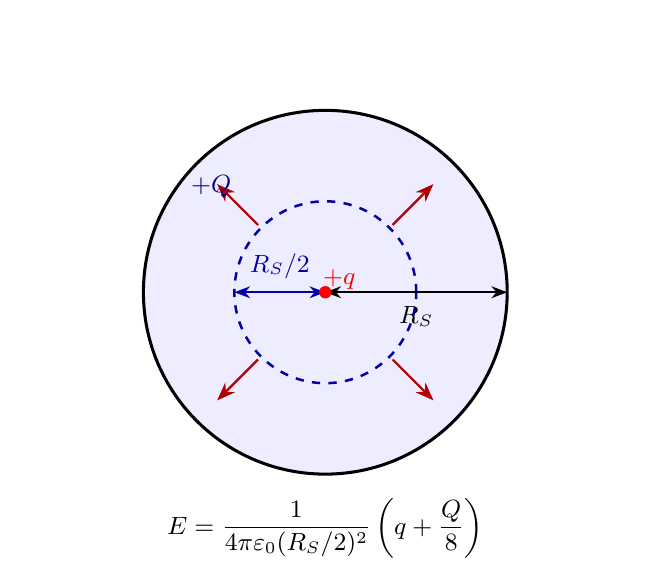
\begin{tikzpicture}[>=Stealth, scale=1.05, every node/.style={font=\small}]
  \useasboundingbox (-3.6,-3.2) rectangle (3.6,3.2);
  % uniformly charged sphere
  \fill[blue!7] (0,0) circle (2.2);
  \draw[line width=1.1pt] (0,0) circle (2.2);
  % gaussian surface at R_S/2
  \draw[line width=0.9pt, dashed, blue!65!black] (0,0) circle (1.1);
  % field arrows (diagonals, clear of the radius arrows)
  \foreach \a in {45,135,225,315} {
    \draw[->, line width=0.8pt, red!70!black] ({1.15*cos(\a)},{1.15*sin(\a)}) -- ({1.85*cos(\a)},{1.85*sin(\a)});
  }
  % radius arrows
  \draw[<->, line width=0.6pt] (0,0) -- (2.2,0) node[midway, below, yshift=-0.05cm] {$R_S$};
  \draw[<->, line width=0.6pt, blue!65!black] (0,0) -- (-1.1,0) node[midway, above, yshift=0.05cm] {$R_S/2$};
  % point charge at centre
  \fill[red] (0,0) circle (0.075);
  \node[red, font=\small\bfseries] at (0.17,0.15) {$+q$};
  % sphere net charge
  \node[blue!55!black, font=\small] at (-1.38,1.28) {$+Q$};
  % result
  \node[font=\small] at (0,-2.85) {$E=\dfrac{1}{4\pi\varepsilon_0 (R_S/2)^2}\left(q+\dfrac{Q}{8}\right)$};
\end{tikzpicture}
\end{document}
